\documentclass{unswmaths}

\usepackage{unswshortcuts}
\usepackage[all]{xy}
\usepackage{csquotes}

\begin{document}

\subject{Algebraic Topology}
\author{Edward McDonald}
\title{Assignment 2}
\studentno{z3375335}

\newcommand{\Hilb}{\mathcal{H}}
\newcommand{\Proj}{\mathbf{P}}
\newcommand{\M}{\mathcal{M}}
\newcommand{\Dom}{\operatorname{Dom}}
\newcommand{\sgn}{\operatorname{sgn}}
\newcommand{\Ha}{\mathcal{H}}
\newcommand{\Span}{\operatorname{span}}
\newcommand{\im}{\operatorname{im}}
\newcommand{\C}{\mathcal{C}}
\newcommand{\D}{\mathcal{D}}
\newcommand{\E}{\mathcal{E}}
\newcommand{\F}{\mathcal{F}}
\newcommand{\G}{\mathcal{G}}
\newcommand{\id}{\mathrm{id}}

\newcommand{\Hom}{\operatorname{Hom}}
\newcommand{\Ab}{\mathbf{Ab}}

\setlength\parindent{0pt}

\unswtitle{}

\section*{Question 1}
\begin{proposition}
    Let $\C$, $\D$ and $\E$ be categories, and $\F:\C\to\D$
    and $\G:\D\to\E$ are functors. Then the composite 
    $\G\F:\C\rightarrow \E$, defined by $(\G\F)(x) = \G(\F(x))$
    for $x \in \operatorname{Obj}(\C)$
    and $(\G\F)(f) = \G(\F(f))$ for a morphism $f$, is a functor.
\end{proposition}
\begin{proof}
    It is necessary to prove,
    \begin{enumerate}
        \item{} If $x \in \operatorname{Obj}(\C)$, then $(\G\F)(\id_{x}) = \id_{\G\F(x)}$.
        \item{} If $f$ and $g$ are morphisms in $\C$ such that $gf$ is defined,
        then $(\G\F)(gf) = (\G\F)(g)(\G\F)(f)$.
    \end{enumerate}
    To prove $1$, we simply compute,
    \begin{align*}
        (\G\F)(\id_x) &= \G(\id_{\F(x)})\\
                      &= \id_{\G\F(x)}.
    \end{align*}
    
    Similarly, we prove $2$, 
    \begin{align*}
        (\G\F)(gf) &= \G(\F(g)\F(f))\\
                   &= (\G\F)(g)(\G\F)(f).
    \end{align*}
\end{proof}

\section*{Question 2}
\begin{lemma}
    Let $f:A\to B$ be a morphism in $\Ab$ that has a left inverse $g:B\to A$. Then
    $f$ is injective and $B$ is the internal direct sum $B = f(A)\oplus \ker g$. 
\end{lemma}
\begin{proof}
    Let $x,y \in A$ with $f(x) = f(y)$. Then $x = g(f(x)) = g(f(y)) = y$, so $f$
    is injective. 
    
    Let $b \in B$. Then
    \begin{equation*}
        b = f(g(b))+(b-f(g(b)))
    \end{equation*}
    See that $g(b-f(g(b))) = g(b)-g(b) = 0$, so $b - f(g(b)) \in \ker(g)$,
    and $f(g(b)) \in f(A)$, so we have the sum $B = f(A) + \ker(g)$. 
    
    To show that this sum is direct, we need to prove that $f(A) \cap \ker(g) = \{0\}$.
    
    To this end, $x \in f(A) \cap \ker(g)$. Then $x = f(y)$ for some $y \in A$.
    Then $0 = g(x) = g(f(y)) = y$. Hence $x = f(0) = 0$. 
\end{proof}


\begin{lemma}
    Let $\C$ and $\D$ be categories, and let $F:\C\to\D$ be a covariant
    functor. If $f \in \Hom_\C(X,Y)$ is left invertible then so is $F(f)$.    
\end{lemma}
\begin{proof}
    Let $g \in \Hom_\C(Y,X)$ be a left inverse for $f$. Then,
    \begin{equation*}
        F(g)F(f) = F(gf) = F(\id_X) = \id_{F(X)}.
    \end{equation*}
    Hence $F(g)$ is a left inverse for $F(f)$.
\end{proof}


Recall that a retract of a topological space $X$ is a subspace $A$
such that the inclusion map $\iota:A\rightarrow X$ is left invertible.

\begin{proposition}
    There is no retract $A$ of the Klein bottle $K$ with $H_1(A) \isom \Itgr^2$.
\end{proposition}
\begin{proof}
    If there were a left invertible map $A\to K$, then there would be a left
    invertible map $\Itgr^2\isom H_1(A)\to H_1(K)\isom \Itgr\oplus \Itgr/2\Itgr$.
    
    Hence there would be an injective map $\varphi:\Itgr^2 \to \Itgr \oplus \Itgr/2\Itgr$. 
    
    Hence there are elements $x,y \in \Itgr\oplus \Itgr/2\Itgr$
    such that there are no non-zero integers $a,b$ such that $xa+yb = 0$. 
    However if $2x = (c,0)$ and $2y = (d,0)$ then 
    
    $2cy - 2dx = 0$. 
    
    Thus $\varphi$ cannot exist, hence $A$ cannot exist.
\end{proof}

\begin{proposition}
    There is no topological space $X$ with $H_1(X) \isom \Itgr^2 \oplus \Itgr/4\Itgr$
    such that the Klein bottle $K$ is a retract of $X$.
\end{proposition}
\begin{proof}
    If $K$ is a retract of $X$. then there is an injection $H_1(K) \to H_1(X)$
    such that the image of $H_1(K)$ is a direct summand of $H_1(X)$. 
    
    
    
    Hence $\Itgr^2 \oplus \Itgr/4\Itgr$ has a subgroup $A \isom \Itgr\oplus \Itgr/2$
    and a subgroup $B$ such that we have the (internal) direct sum 
    $\Itgr^2 \oplus \Itgr/4\Itgr = A\oplus B$. 
    
%    Hence
%    $(0,0,1) \in B$. But then $(0,0,2) = (0,1) + (0,1) \in B$. However $(0,2)$ is the only
%    element of $\Itgr^2 \oplus \Itgr/4\Itgr$ that is of order $2$. Since $A$ must 
%    have an element of order $2$, we conclude that the decomposition 
%    $\Itgr^2\oplus \Itgr/4\Itgr = A\oplus B$ is impossible.
 
    See that $\Itgr^2\oplus \Itgr/4\Itgr$ has a unique element of order $2$,
    $(0,0,2)$. Since $A$ must have an element of order $2$, we conclude
    that $(0,0,2) \in A$. 
    

    Note that $A$ has no element of order $4$, hence $(0,0,1) \notin A$. 
    Hence there is some nonzero $b \in B$ such that $b-(0,0,1) \in A$. 
    
    Thus $2b - (0,0,2) \in A$, hence $2b \in A$. But $b \in B$, so $2b \in B \cap A$.
    Hence $b = 0$, so $(0,0,1) \in A$, which is a contradiction.

    
\end{proof} 





\section*{Question 3}
\begin{proposition}
    Let $f:S^n\to S^n$ be a continuous function with non-zero degree.
    Then $f$ is surjective.
\end{proposition}
\begin{proof}
    Let $f:S^n\to S^n$ be a continuous function that is not surjective. 
    Let $y \in S^n$ be not in the image of $f$. Let $p:S^n\rightarrow \Rl^n$
    be stereographic projection from the point $y$. Consider
    the functions $r:[0,1]\times \Rl^n\rightarrow \Rl^n$ that contracts by $t$,
    $r(t,x) = (1-t)x$. $r$ is a polynomial so $r$ is continuous. 
    
    Then $H(t,x) = p^{-1}(r(t,p(f(x))))$ continuous, and
    $H(0,x) = p^{-1}(p(f(x)) = f(x)$, 
    and $H(1,x) = p^{-1}(0)$. Thus $H$ is a homotopy of $f$ to a constant map.
    
    Hence $f$ is homotopic to a constant map, so $\deg(f) = 0$.
\end{proof}

\section*{Question 4}
We consider $S^{n-1}$ as a subset of $S^n$ by embedding it into the equator.

\begin{proposition}
    The relative homology $H_p(S^n,S^{n-1})$ is as follows:
    \begin{equation*}
        H_p(S^n,S^{n-1}) \isom \begin{cases}
            \Itgr^2,\;p = n\\
            0,\text{ otherwise.}
        \end{cases}
    \end{equation*}
\end{proposition}
\begin{proof}
    We shall compute the homology with a specific triangulation of $S^n$. Let $\sigma_1,\sigma_2,\sigma_3$
    be three distinct $n$-simplices, and let $w,w'$ be two vertices
    not in $\sigma_i$,$i = 1,2,3$.
    
    We construct a triangulation $K$ as follows:\\    
    Place $\sigma_2$ at the equator of $S^n$, and put $\sigma_1$
    and $\sigma_3$ below and above $\sigma_2$ respectively. 
    
    Place the vertex $w$ on the surface of the sphere, beneath
    $\sigma_1$, and $w'$ is the antipodal point to $w$ above $\sigma_3$. 
    Now we connect $K_{\sigma_1}^{(n-1)}*w$ to $\sigma_2$ as illustrated
    below in the case for $n = 2$,\\
    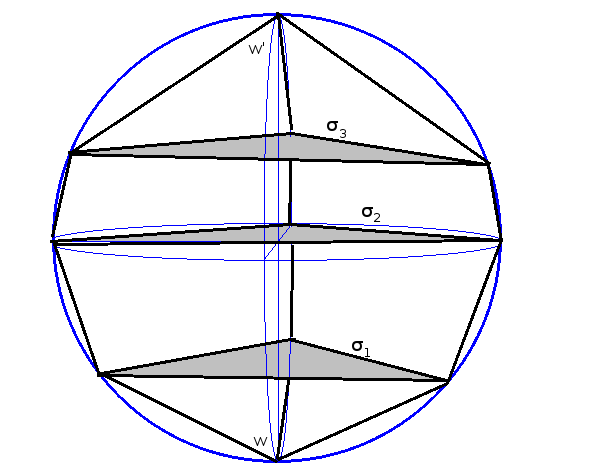
\includegraphics[width=100mm]{artwork/sphere.png}\\
    similarly $K_{\sigma_3}^{(n-1)}*w'$ is connected to $\sigma_2$. 
    
    Thus we have a triangulation $K$ of $S^n$, and  $K_{\sigma_2}^{(n-1)}$
    corresponds to $S^{n-1}$.
    
    Now let $p > 0$. We need to compute $C_p(K)/C_p(K_{\sigma_2}^{(n-1)})$.
    
    Let $L$ be the simplicial complex that is the image of $K$ 
    where all of $K_{\sigma_2}^{n-1}$ is identified to a point $x \in L$. 
    
    We claim that there is an isomorphism $C_p(L) \isom C_p(K)/C_p(K_{\sigma_2}^{(n-1)})$.
    
    Let $\varphi:C_p(K)\rightarrow C_p(L)$ be the map that sends
    simplices in $K_{\sigma_2}^{(n-1)}$ to $0$. Hence $\ker\varphi = C_p(K_{\sigma_2}^{(n-1)})$,
    so we have the required isomorphism.
    
    It is then easy to see that the boundary map $\partial_p$
    is the same on $C_p(L)$ as it is on $C_p(K)/C_p(K_{\sigma_2}^{(n-1)}$. 
    Hence the relative homology $H_p(S^n,S^{n-1})$
    is the same as the homology $H_p(L)$ for $p > 0$.
    
    Now $L$ is a union of two $n$-spheres, so we have $H_p(L) = 0$
    for $0 < p < n$ and $H_n(L) = \Itgr^2$. 
    
    For the case $p = 0$, we consider $C_0(K)/C_0(K_{\sigma_2}^{(n-1)})$. Now $Z_0(K,K^{(n-1)}_{\sigma_2}) = C_0(K)/C_0(K_{\sigma_2}^{(n-1)})$.
    
    However, for every vertex $x \in K \setminus K_{\sigma_2}^{(n-1)}$, there is a one
    chain joining a vertex in $K_{\sigma_2}^{(n-1)}$ to $x$. Hence
    every point $x \in K \setminus K_{\sigma_2}^{(n-1)}$ is the $0$-boundary
    of a $1$-chain, modulo points of $K_{\sigma_2}^{(n-1)}$. Hence $H_0(S^n,S^{n-1}) \isom 0$.
\end{proof}

\section*{Question 5}
Let $X = \Rl^2\setminus \{p,q\}$ for distinct points $p,q \in \Rl^2$. 
Let $A$ be the union of the circles centred at $p$ and $q$
with radius half the distance between $p$ and $q$.
\begin{proposition}
    $A$ is a weak deformation retract of $X$. 
\end{proposition}
\begin{proof}
    By a change of coordinates, we can set
    $p = (1,0)$ and $q = (-1,0)$. Let $C_p$ be the disc centred at
    $p$ with radius $1$, and $C_q$ is similarly the disc centred at $q$
    with radius $1$.

    First we note that the relation of being a weak deformation
    retract is transitive, in the sense that if $A \subseteq B \subseteq X$
    is a nested triple of topological spaces,
    and $B$ is a weak deformation retract of $X$, and $A$ is a weak deformation
    retract of $B$, then $A$ is a weak deformation
    retract of $X$. 
    
    Let $D$ be the closed disc centred at $(0,0)$ of radius $2$. 
    
    It is easy to see that $D\setminus \{p,q\}$ is a weak deformation
    retract of $X$, simply project the exterior of $D$ onto $D$.
    
    Now we show that $A$ is a weak deformation retract of $D$. 
    
    We now define a function $H:[0,1]\times D\rightarrow D$.
    Let $H$ move points outside of $C_p\cup C_q$ onto
    the boundary of $C_p \cup C_q$ by moving them towards the $x$-axis. 
    
    For a point $a \in C_p \setminus \{p\}$, let $H$ radially
    move $a$ towards the boundary of $C_p$. Similarly $H$
    moves points in $C_q$
    towards the boundary of $C_q$.
    
\end{proof}

\begin{proposition}
    We can triangulate $A$ as follows:\\
    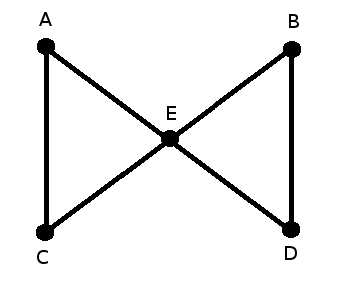
\includegraphics[width=90mm]{artwork/triang.png}\\
    Let $K$ be the associated simplicial complex.
\end{proposition}
\begin{proof}
    Simply perform a projection from $|K|$ to $A$.
\end{proof}

\begin{proposition}
    The homology of $A$ is
    \begin{equation*}
        H_p(A) \isom \begin{cases}
            \Itgr^2,\;p = 1\\
            \Itgr,\;p = 0\\
            0\text{ otherwise.}
        \end{cases}
    \end{equation*}
\end{proposition}
\begin{proof}
    By the main theorem of the course, $H_p(A) = H_p(K)$. Since $K$
    has no $p$-simplices for $p \neq 0,1$, the only potentially
    non-trivial homology groups are $H_1(K)$ and $H_0(K)$. 
    
    Since $K$ is connected, we have $H_0(K) \isom \Itgr$.
    
    So we now need only compute $H_1(K)$. Since $C_2(K) = 0$,
    this is exactly $Z_1(K)$. Let $a \in Z_1(K)$. Write,
    \begin{equation*}
        a = \sum_{\sigma}a_{\sigma}\sigma
    \end{equation*}
    where the sum runs over all $1$-simplices in $K$. Since $\partial a = 0$, 
    we have that $a_{AC} = a_{CE} = a_{AE}$ and $a_{EB} = a_{BD} = a_{DE}$. Hence
    $Z_1(K)$ is generated by the $1$-chains $[AC]+[CE]+[AE]$ and $[EB]+[BD]+[DE]$. No
    multiple of these chains can be zero, so we have two order zero generators of $Z_1(K)$. 
    Since they are independent over $\Itgr$, we have $H_1(K) \isom \Itgr^2$.
\end{proof}

\begin{proposition}
    $\Rl^2 \setminus \{p,q\}$ is not homeomorphic to $\Rl^2 \setminus \{p\}$.
\end{proposition}
\begin{proof}
    It was proved in class that $\Rl^2 \setminus \{p\}$ is a weak deformation retract of $S^1$.
    Hence $H_1(\Rl^2\setminus \{p\}) = \Itgr$. Thus $\Rl^2\setminus \{p\}$ and $\Rl^2\setminus\{p,q\}$
    have different homology.
\end{proof}

\end{document}
